%!TEX root = ../PhD_thesis__Lilian_Besson

\chapter{SMPyBandits: a state-of-the-art Python library to simulate MAB problems}
\label{chapter:3}
\minitoc

SMPyBandits is a package I have developed since the beginning of my PhD.
It is designed to allow easy and efficient numerical simulations on single-player and multi-players Multi-Armed Bandits (MAB) algorithms, and SMPyBandits is written in Python.
This library is by far the most complete open-source implementation of state-of-the-art algorithms tackling various kinds of MAB sequential learning problems.
It aims at being extensive, simple to use and maintain, with a clean and well documented codebase.
It allows fast prototyping of simulations and experiments, with an easy configuration system and command-line options to customize experiments.
Experiment results are saved in an optimized binary format (HDF5) as well as high quality plots of many useful visualizations.
%
More than two years of active development have shown how easy it can be to add new algorithms, new arm distributions, and new bandit models (\eg, Markov or non-stationary).

This chapter details the organization of the library, what it implements in terms of arm distributions, models, algorithms and visualizations.
Then we use it to perform a numerical comparisons of the main state-of-the-art single-player MAB algorithms, as well as a study to compare time and memory costs of the main algorithms.
% \TODOL{Do we really have time/space to talk about Markov models?}
% Finally, we introduce rested or restless Markov models and use the library to simulate and illustrate the performance of the classical \UCB{} algorithm.

% \newpage
% Write miniTOC just after the title
\graphicspath{{2-Chapters/3-Chapter/Images/}}
\graphicspath{{2-Chapters/3-Chapter/SMPyBandits_paper.git/plots/}}

% This chapter is intended as a long version of the paper presenting SMPyBandits that I wrote in Summer 2018, see https://hal.inria.fr/hal-01840022

SMPyBandits is the most complete open-source implementation of state-of-the-art algorithms tackling various kinds of sequential learning problems referred to as Multi-Armed Bandits.
It aims at being extensive, simple to use and maintain, with a clean and perfectly documented codebase. But most of all it allows fast prototyping of simulations and experiments, with an easy configuration system and command-line options to customize experiments while starting them (see below for an example).

SMPyBandits does not aim at being blazing fast or optimal in terms of memory usage, and it comes with a pure Python implementation \cite{python}, with no dependency except standard open-source Python packages.
Even if some critical parts are also available as a \texttt{C} Python extension, and even by using Numba \cite{numba} whenever it is possible, if simulation speed really matters, one should rather refer to less exhaustive but faster implementations, like for example \cite{TorLibbandit} in \texttt{C++} or \cite{VishMABjl} in Julia.

In this Chapter~\ref{chapter:3}, we start by presenting in Section~\ref{sec:3:presentationLibrary} the organization of the library.
We use the library to compare the most famous and most efficient single-player MAB algorithms in Section~\ref{sec:3:reviewSPAlgorithms},
then we present in Section~\ref{sec:3:timeAndMemoryCosts} additional numerical simulations to discuss about the time efficient and memory costs of the some MAB algorithms (we focus on the ones being used in the rest of this thesis, \UCB, \klUCB, and Thompson Sampling).
To also illustrate how one can easily extend the SMPyBandits library to add not only add new distributions or new algorithms, but also new bandit models, we detail in Section~\ref{sec:3:markovModels} how we added the possibility to simulate Markovian models (as introduced by \cite{Anantharam87b}).
%
Finally, in Appendix~\ref{sec:3:appendix} we include some minimalist files showing how to use the library, as well as details regarding the possible use of multiple cores to speed-up simulations.


\paragraph{Publications}
%
This chapter is based on the following publication: \cite{SMPyBanditsJMLR}.
The code for SMPyBandits is hosted online at \texttt{\href{https://GitHub.com/SMPyBandits/SMPyBandits/}{GitHub.com/SMPyBandits/SMPyBandits}}, its documentation is at \texttt{\href{https://SMPyBandits.GitHub.io/}{SMPyBandits.GitHub.io}} or \texttt{\href{https://SMPyBandits.RTFD.io/}{SMPyBandits.RTFD.io}}, and all the library is publicly released under the MIT open-source License.


% ----------------------------------------------------------------------------
\section{Presentation of the library}
\label{sec:3:presentationLibrary}

% I want to show what is SMPyBandits, what problems does it solve, what did I implement, how to use it.

We start by explaining how SMPyBandits simulates MAB problems, by detailing the different parts.
We then detail how SMPyBandits implements MAB algorithms (\eg, \UCB),
and what kind of information is displayed, saved and plotted after a batch of simulations of bandit problems.

The main goal of the library is to be easily able to simulate a small number of algorithms (\eg, three algorithms like \UCB, \klUCB{} and Thompson sampling) on one or more bandit models (single- or multi-player) defined by the number of arms $K$ and the distributions $\nu_k$, for some time from $t=1$ to the horizon $T$.
After the simulation, the library then displays statistical summary of the (mean) rewards accumulated by each algorithms, as well as regret and other visualizations.
The same problem is simulated for $N$ independent repetitions (\eg, $N=1000$) in order to show mean results with a low variance.


\subsection{Single- and multi-player MAB problems}

For the classical single-player stochastic MAB model, as defined in Chapter~\ref{chapter:2},
a stochastic MAB problem is defined by $K>1$ distributions $\nu_k$ (also called arms),
used to sample \iid{} rewards $r_k(t) \sim \nu_k, \forall t$.
An agent choose arm $A(t)\in\{1,\dots,K\}$ at time $t$ and observes the reward $r_{A(t)}(t)$ without knowing the other (hidden) rewards.
Her goal is to maximize $\sum_{t=1}^T r_{A(t)}(t)$ by sequentially exploring the $K$ arms, and she essentially has to find and exploit the best one as fast as possible.

\paragraph{Simulation loop}
%
Any simulation library targeting single-player bandit problems must implement at least three components:
reward distributions, MAB algorithm, and a simulation loop that essentially looks like this.
\begin{itemize}
    \item First, initialize the MAB problem and one or more algorithms,
    \item Then, for $t=1$ to $t=T$ (known before hand), repeat the following block (for each algorithm). Ask algorithm $\cA$ his chosen arm $A(t)$, then sample a (random) reward $r(t)$ (\iid) from distribution $\nu_{A(t)}$, and finally feeds the observation $(A(t), r(t))$ to the algorithm,
    \item At the end, compute the accumulated reward, the regret, plot visualizations etc.
\end{itemize}
%
Note that the second step should of course be repeated a large number of times if we want to study \emph{mean} regret and not only the regret in one single trajectory.
If one wants to compare algorithms on a same problem, it is possible to sample all the rewards $(r_k(t))_{k\in[K], t\in[T]}$ before-hand, and store them so that for each repetition of the simulation, the randomness from the environment (\ie, the rewards) has the same impact on all the algorithms.


\paragraph{Simulation loop for multi-player bandit}

For Cognitive Radio and other applications, a well-studied extension is to consider $M\geq2$ players, interacting on the same $K$ arms.
Whenever two or more players select the same arm at the same time, they all suffer from a collision.
%
Different collision models has been proposed, and the simplest one consists in giving a $0$ reward to each colliding players.
Without any centralized supervision or coordination between players, they must learn to access the $M$ best resources (\ie, arms with highest means) without collisions.
We refer to Chapter~\ref{chapter:5} which introduces and details various multi-player bandit models.

SMPyBandits implements all collision models found in the literature (in the module \texttt{\href{https://SMPyBandits.GitHub.io/docs/Environment.CollisionModels.html}{Environment.CollisionModels}}), as well as all the algorithms known by the authors (in the module \texttt{\href{https://SMPyBandits.GitHub.io/docs/Environment.CollisionModels.html}{Environment.CollisionModels}}).
%
It includes
\texttt{rhoRand} (\texttt{\href{https://SMPyBandits.GitHub.io/docs/PoliciesMultiPlayers.rhoRand.html}{PoliciesMultiPlayers.rhoRand}}) from \cite{Anandkumar11},
\texttt{MEGA} (\texttt{\href{https://SMPyBandits.GitHub.io/docs/Policies.MEGA.html}{Policies.MEGA}}) from \cite{Avner15},
\texttt{MusicalChair} (\texttt{\href{https://SMPyBandits.GitHub.io/docs/Policies.MusicalChair.html}{Policies.MusicalChair}}) from \cite{Rosenski16},
and our state-of-the-art algorithms
\texttt{RandTopM} (\texttt{\href{https://SMPyBandits.GitHub.io/docs/PoliciesMultiPlayers.RandTopM.html}{PoliciesMultiPlayers.RandTopM}}) and
\texttt{MCTopM} (\texttt{\href{https://SMPyBandits.GitHub.io/docs/PoliciesMultiPlayers.MCTopM.html}{PoliciesMultiPlayers.MCTopM}}) from \cite{Besson2018ALT}.
For comparison, realistic (\eg, \UCB{} for multiple play) or full-knowledge centralized algorithms are also implemented.

Any simulation library targeting multi-player bandit problems must implement at least another component:
a collision model, and a simulation loop that essentially looks like this.
\begin{itemize}
    \item First, initialize the MAB problem with $M$ players, and one or more cohorts of $M$ players (one player is one algorithm, usually $M$ times the same one),
    \item Then, for $t=1$ to $t=T$ (known before hand), repeat the following block (for each algorithm). Ask each player $\cA^{(j)}$ his chosen arm $A^{(j)}(t)$, then query the collision model\footnote{~The default collision model is the most widely studied in the literature, where a player encounters a collision (\ie, received a zero reward $Y^{(j)}(t)=0$) if she is not the only one to have chosen an arm $k=A^{(j)}(t)$, otherwise $Y^{(j)}(t)=r_{A^{(j)}(t)}(t)$ if she is the only one playing this arm.} to know which player will get a zero reward (for a collision) and which player will get a random reward from the environment. The
    sample (random) feedback $r_k(t)$ (\iid) from distributions $\nu_{k}$, and compute the rewards $Y^{(j)}(t)$ from the random feedback and the collision model. Finally feeds the observation $(A^{(j)}(t),Y^{(j)}(t))$ to the $M$ players,
    \item At the end, compute the accumulated reward, the regret, plot visualizations etc.
\end{itemize}


\subsection{Reward distributions}
%
This library tackles one dimensional distributions,
and supports \emph{Bernoulli} (\texttt{\href{https://smpybandits.github.io/docs/Arms.Bernoulli.html}{Arms.Bernoulli}}), \emph{binomial} (\texttt{\href{https://smpybandits.github.io/docs/Arms.Binomial.html}{Arms.Binomial}}), \emph{Poisson} (\texttt{\href{https://smpybandits.github.io/docs/Arms.Poisson.html}{Arms.Poisson}}), and a generic \emph{discrete} (\texttt{\href{https://smpybandits.github.io/docs/Arms.DiscreteArm.html}{Arms.DiscreteArm}}) distributions,
as well as \emph{exponential} (\texttt{\href{https://smpybandits.github.io/docs/Arms.Exponential.html}{Arms.Exponential}}), \emph{gamma} (\texttt{\href{https://smpybandits.github.io/docs/Arms.Gamma.html}{Arms.Gamma}}), \emph{Gaussian} (\texttt{\href{https://smpybandits.github.io/docs/Arms.Gaussian.html}{Arms.Gaussian}}) and \emph{uniform} (\texttt{\href{https://smpybandits.github.io/docs/Arms.Uniform.html}{Arms.Uniform}}) continuous distributions,
which can be truncated to an interval $[a,b]$ or have unbounded support ($\mathbb{R}$).
%
The default is to use the same distribution for the $K$ arms, but it also possible to mix them (see for instance Figure~\ref{fig:25:HarderMixed}).
%
We do not give more details, but the interested reader can refer to the following Jupyter notebook \cite{jupyter} document hosted at:\\
\begin{small}
    \href{https://smpybandits.github.io/notebooks/Easily_creating_MAB_problems.html}{\texttt{SMPyBandits.GitHub.io/notebooks/Easily\_creating\_MAB\_problems.html}}
\end{small}


\subsection{MAB algorithms}

SMPyBandits is a complete open-source implementation of single-player (classical) bandit algorithms,
containing over 65 (in the module \texttt{\href{https://SMPyBandits.GitHub.io/docs/Policies.html}{Policies}}) algorithms.
It uses a well-designed hierarchical structure and class inheritance scheme (as detailed on the various UML diagrams showed on the \texttt{\href{https://SMPyBandits.GitHub.io/uml_diagrams/README.html}{uml\_diagrams}} folder) to minimize redundancy in the codebase.
For instance, most existing algorithms are index-based, and new ones can be written easily by inheriting from the \texttt{IndexPolicy} class (\texttt{\href{https://SMPyBandits.GitHub.io/docs/Policies.IndexPolicy.html}{Policies.IndexPolicy}}).
An index-based algorithm computes an index $I_k(t)\in\mathbb{R}$ for each arm $k$ at time $t$ and simply play $A(t) = \arg\max_k I_k(t)$.
For instance the code specific to the UCB algorithm \cite{LaiRobbins85,Auer02} is as short as this (and fully documented):

% https://tex.stackexchange.com/a/12430/
\begin{small}
% \begin{listing}[h!]
    \inputminted[linenos=true,numbersep=5pt,frame=lines,framesep=2mm]{python3}{2-Chapters/3-Chapter/src/example_of_a_IndexPolicy_UCB.py}
    % \caption{Small snippet of code defining the UCB algorithm, as a simple example of an Index Policy}
    \captionof{listing}{Small snippet of code defining the UCB algorithm, as a simple example of an Index Policy \label{lst:3:smallIndexPolicy}.}
    % \label{lst:3:smallIndexPolicy}
% \end{listing}
\end{small}


\subsubsection{Features}

With this numerical framework, simulations can run on a single CPU or a multi-core machine using joblib \cite{joblib},
and summary plots are automatically saved as high-quality PNG, PDF and EPS, using matplotlib \cite{matplotlib} and seaborn \cite{seaborn}.
Raw data from each simulation is also saved in a HDF5 file using h5py \cite{h5py}, an efficient and compressed binary format, to allow easy post-mortem exploration of simulation results.
Making new simulations is very easy, one only needs to write a configuration script (\texttt{configuration.py}), without needing a complete knowledge of the internal code architecture.

A complete Sphinx documentation, for each algorithm and all parts of the codebase, even including the constants in the different configuration files, is available here: \texttt{\href{https://SMPyBandits.GitHub.io}{SMPyBandits.GitHub.io}}.


\subsubsection{How to run experiments?}

We show how to install SMPyBandits, and an example of how to run a simple experiment.
This bash snippet\footnote{~See this page \texttt{\href{https://SMPyBandits.GitHub.io/How_to_run_the_code.html}{SMPyBandits.GitHub.io/How\_to\_run\_the\_code.html}} for more details.} shows how to clone the code\footnote{~SMPyBandits is also available on Pypi, see \texttt{\href{https://pypi.org/project/SMPyBandits/}{pypi.org/project/SMPyBandits}}. You can install it directly with \texttt{sudo pip install SMPyBandits}, or from a \texttt{virtualenv} \cite{virtualenv}.},
and install the requirements for Python 3 (once):

% https://tex.stackexchange.com/a/12430/
\begin{small}
    \begin{listing}[h!]
        \begin{minted}[linenos=true,numbersep=5pt,frame=lines,framesep=2mm]{bash}
# 1. get the code in the folder you want
$ git clone https://GitHub.com/SMPyBandits/SMPyBandits.git
$ cd SMPyBandits.git
# 2. install the requirements
$ pip install -r requirements.txt
        \end{minted}
        \caption{Small snippet of Bash to download and install dependencies of SMPyBandits}
        % \captionof{listing}{Small snippet of Bash to download and install dependencies of SMPyBandits \label{lst:3:howToInstallLibrary}.}
        \label{lst:3:howToInstallLibrary}
    \end{listing}
\end{small}

Launching simulations is easy, for instance this snippet shows how to start $N=1000$ repetitions of a simple non-Bayesian Bernoulli-distributed problem, for $K=9$ arms, an horizon of $T=10000$ and on $4$ CPUs.
It takes about $20$ minutes, on a standard $4$-cores $64$ bits GNU/Linux laptop.
Using environment variables (\texttt{N=1000} etc) in the command line is not required, but it is convenient:

% https://tex.stackexchange.com/a/12430/
\begin{small}
\begin{listing}[h!]
    \begin{minted}[linenos=true,numbersep=5pt,frame=lines,framesep=2mm]{bash}
# 3. run a single-player simulation
$ BAYES=False ARM_TYPE=Bernoulli N=1000 T=10000 K=9 N_JOBS=4 \
  MEANS=[0.1,0.2,0.3,0.4,0.5,0.6,0.7,0.8,0.9] \
  python3 main.py configuration.py
    \end{minted}
    \caption{Small snippet of Bash to run a simple experiment with SMPyBandits}
    % \captionof{listing}{Small snippet of Bash to run a simple experiment with SMPyBandits \label{lst:3:howToRunBasicLibrary}.}
    \label{lst:3:howToRunBasicLibrary}
\end{listing}
\end{small}


\subsection{Example of a simulation and illustration}

A small script \texttt{configuration.py} (\texttt{\href{https://SMPyBandits.GitHub.io/docs/configuration.html}{SMPyBandits.GitHub.io/docs/configuration.html}}) is used to import the arm classes (\texttt{\href{https://SMPyBandits.GitHub.io/docs/Arms.html}{SMPyBandits.GitHub.io/docs/Arms.html}}), the policy classes (\texttt{\href{https://SMPyBandits.GitHub.io/docs/Policies.html}{SMPyBandits.GitHub.io/docs/Policies.html}}) and define the problems and the experiments.
Choosing the algorithms is easy by customizing the \texttt{configuration["policies"]} list in the \texttt{configuration.py} file.
For instance, one can compare the standard anytime \klUCB{} algorithm (class \texttt{\href{https://SMPyBandits.GitHub.io/docs/Policies.klUCB.html}{Policies.klUCB}}) against the non-anytime variant $\klUCB^{++}$ algorithm (\texttt{\href{https://SMPyBandits.GitHub.io/docs/Policies.klUCBPlusPlus.html}{Policies.klUCBPlusPlus}}), and also \UCB{} with $\alpha=1$ (\texttt{\href{https://SMPyBandits.GitHub.io/docs/Policies.UCBalpha.html}{Policies.UCB}}) and Thompson sampling (\texttt{\href{https://SMPyBandits.GitHub.io/docs/Policies.Thompson.html}{Policies.Thompson}}) with a Beta posterior (\texttt{\href{https://SMPyBandits.GitHub.io/docs/Policies.Posterior.Beta.html}{Policies.Posterior.Beta}})).

% https://tex.stackexchange.com/a/12430/
\begin{small}
\begin{listing}[h!]
    \begin{minted}[linenos=true,numbersep=5pt,frame=lines,framesep=2mm]{python3}
configuration["policies"] = [
  {"archtype": klUCB, "params": {"klucb": klucbBern}},
  {"archtype": klUCBPlusPlus, "params": {"horizon": HORIZON, "klucb": klucbBern}},
  {"archtype": UCBalpha, "params": {"alpha": 1}},
  {"archtype": Thompson, "params": {"posterior": Beta}}
]
    \end{minted}
    \caption{Small snippet of Python code to configure the list of algorithms tested on a problem.}
    % \captionof{listing}{Small snippet of Python code to configure the list of algorithms tested on a problem. \label{lst:3:howToConfigureAlgorithms}.}
    \label{lst:3:howToConfigureAlgorithms}
\end{listing}
\end{small}

\begin{figure}[h!]  % [htbp]
	% \centering
	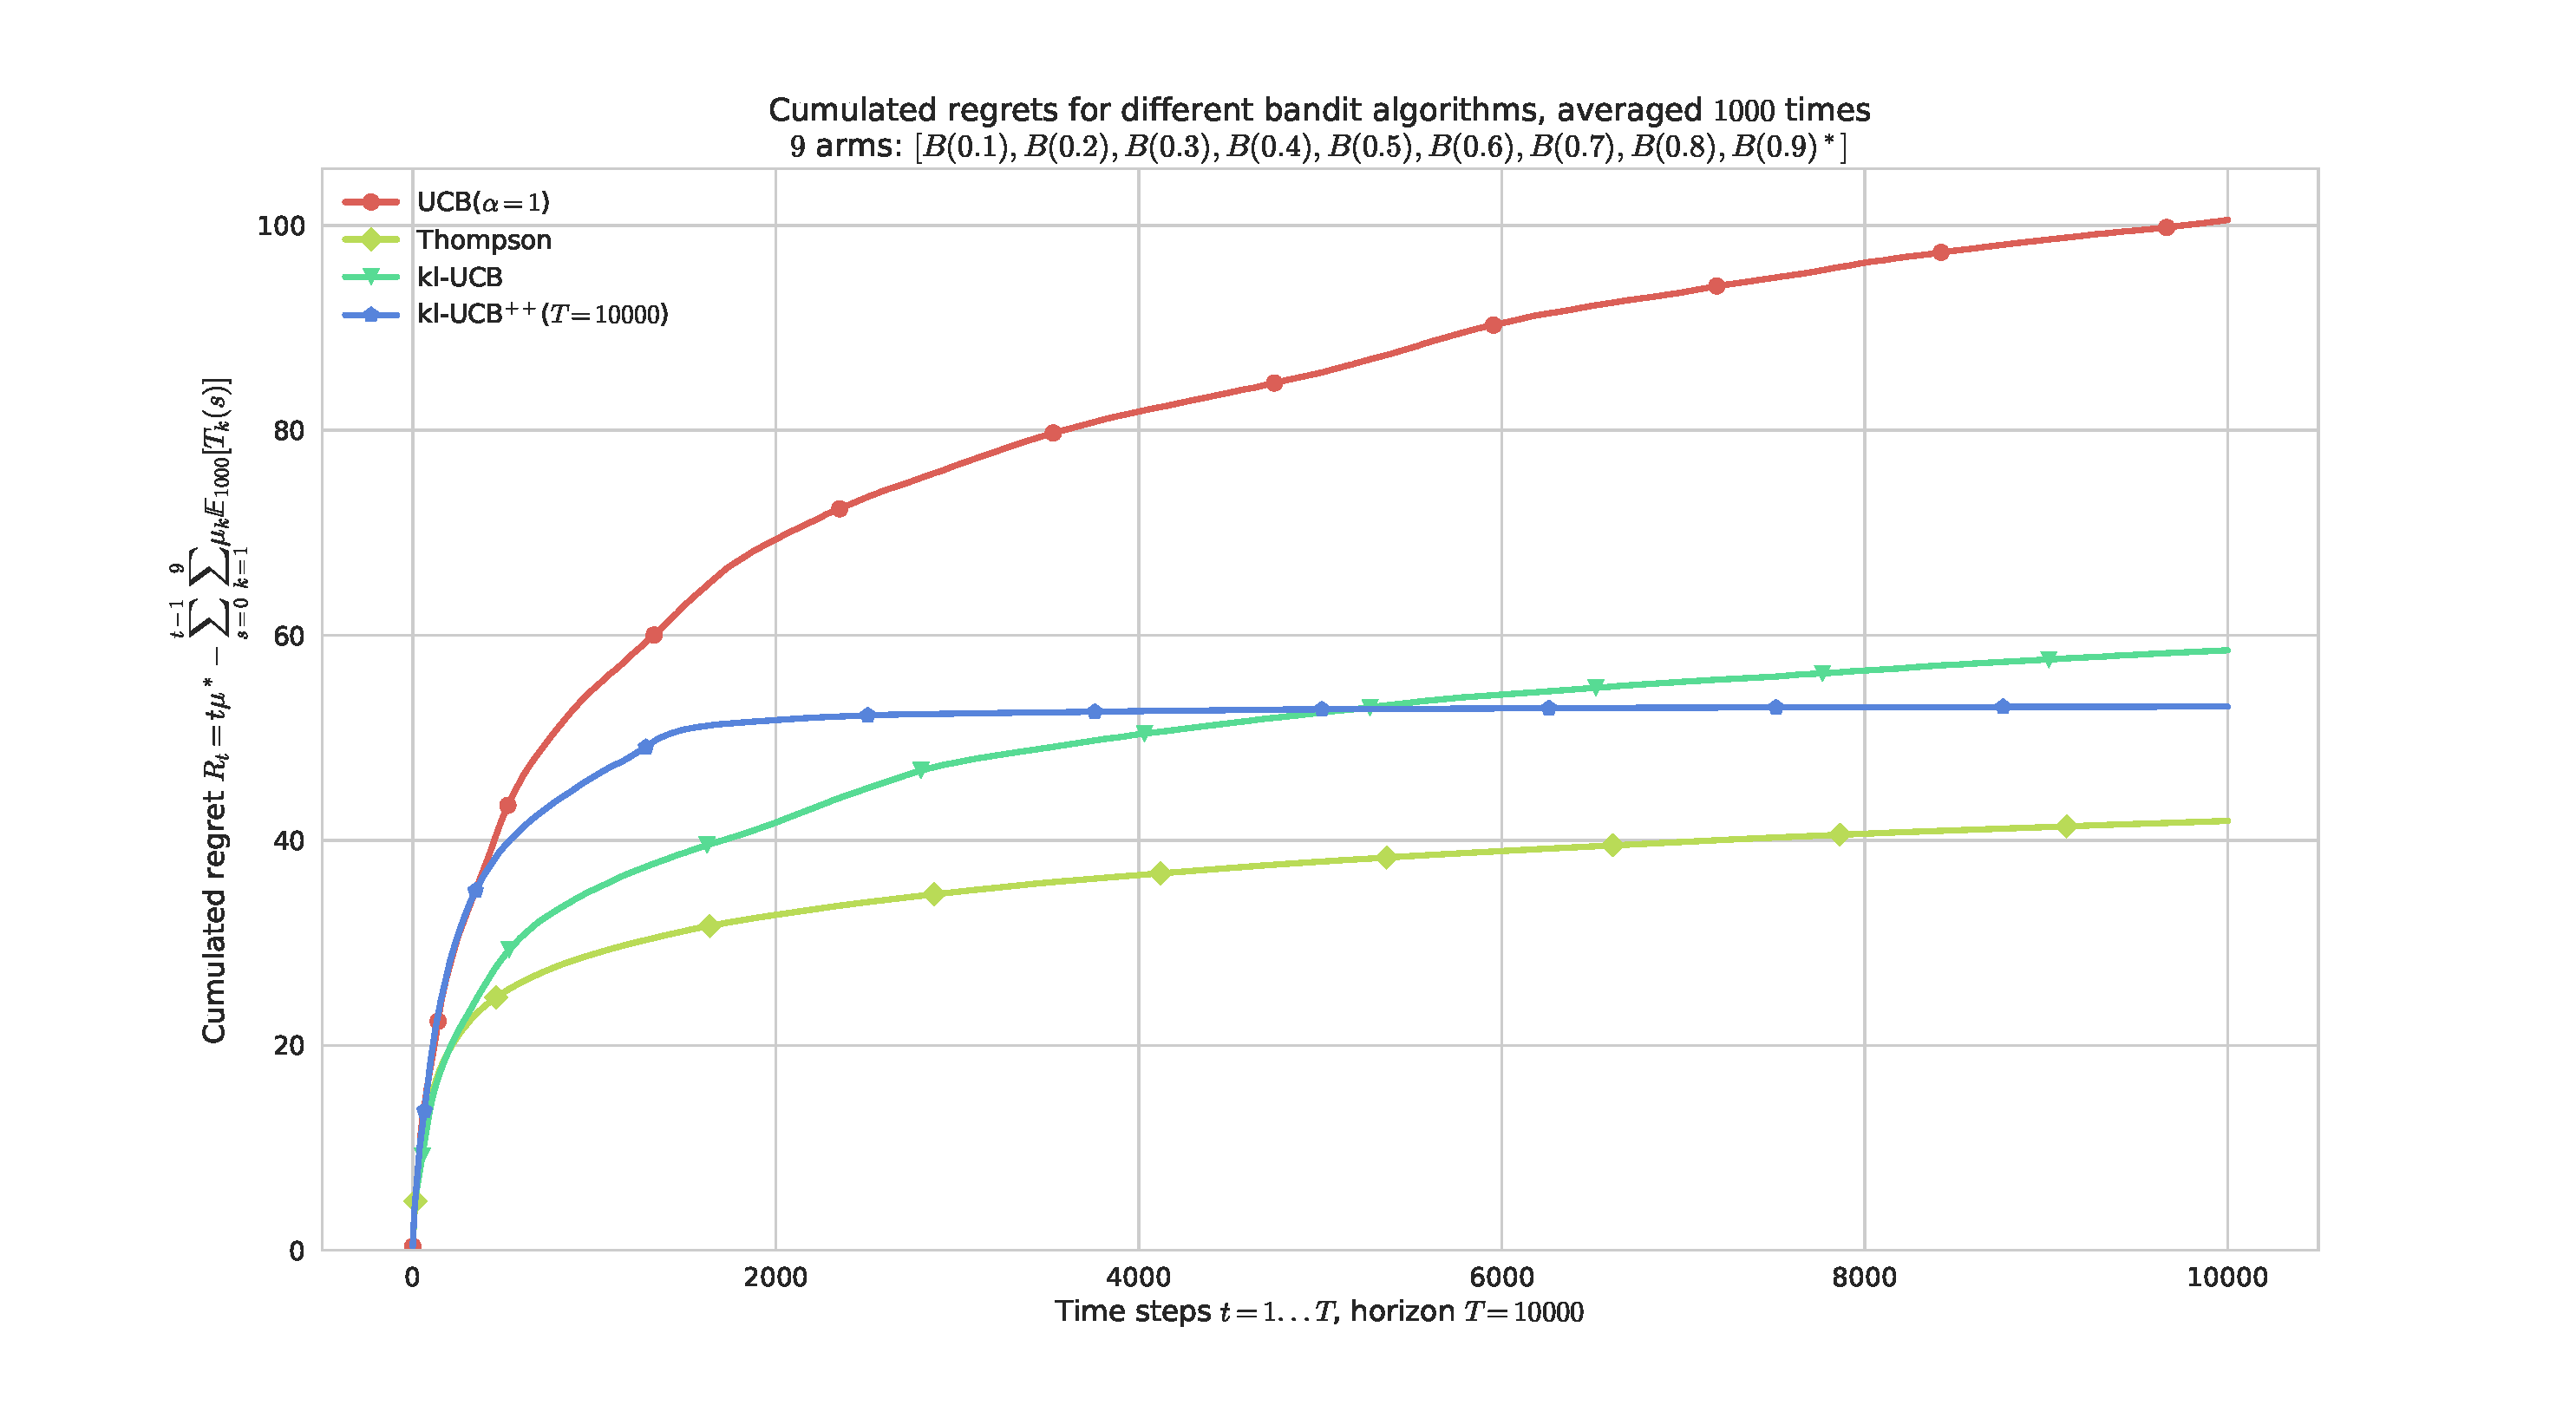
\includegraphics[width=1.05\linewidth]{3.pdf}
	\caption[Example of a single-player simulation showing the average regret and histogram of regrets of $4$ algorithms]{
		Example of a single-player simulation showing the average regret and histogram of regrets of four algorithms. They all perform very well: each algorithm is known to be order-optimal (\ie, its regret is proved to match the lower-bound up-to a constant), and each but UCB is known to be optimal (\ie, with the constant matching the lower-bound). For instance, Thomson sampling is very efficient in average (in yellow), and UCB shows a larger variance (in red).
	}
	\label{fig:3:firstPlot}
\end{figure}

Running the simulation as shown above will save figures in a sub-folder, as well as save data (pulls, rewards and regret) in a HDF5 file\footnote{~For example, this simulation produces this HDF5 file\\\texttt{\href{https://github.com/SMPyBandits/SMPyBandits/blob/master/plots/paper/example.hdf5}{GitHub.com/SMPyBandits/SMPyBandits/blob/master/plots/paper/example.hdf5}}}
\cite{h5py}.
% \texttt{\href{http://docs.h5py.org/en/stable/high/file.html}{docs.h5py.org/en/stable/high/file.html}}).
Figure~\ref{fig:3:firstPlot} above shows the average regret for these $4$ algorithms.
The regret is the difference between the cumulated rewards of the best fixed-armed strategy (which is the oracle strategy for stationary bandits), and the cumulated rewards of the considered algorithms.
The Figure~\ref{fig:3:firstPlot_hist} below shows the histogram of regret for the same experiment.

\begin{figure}[h!]  % [htbp]
	% \centering
	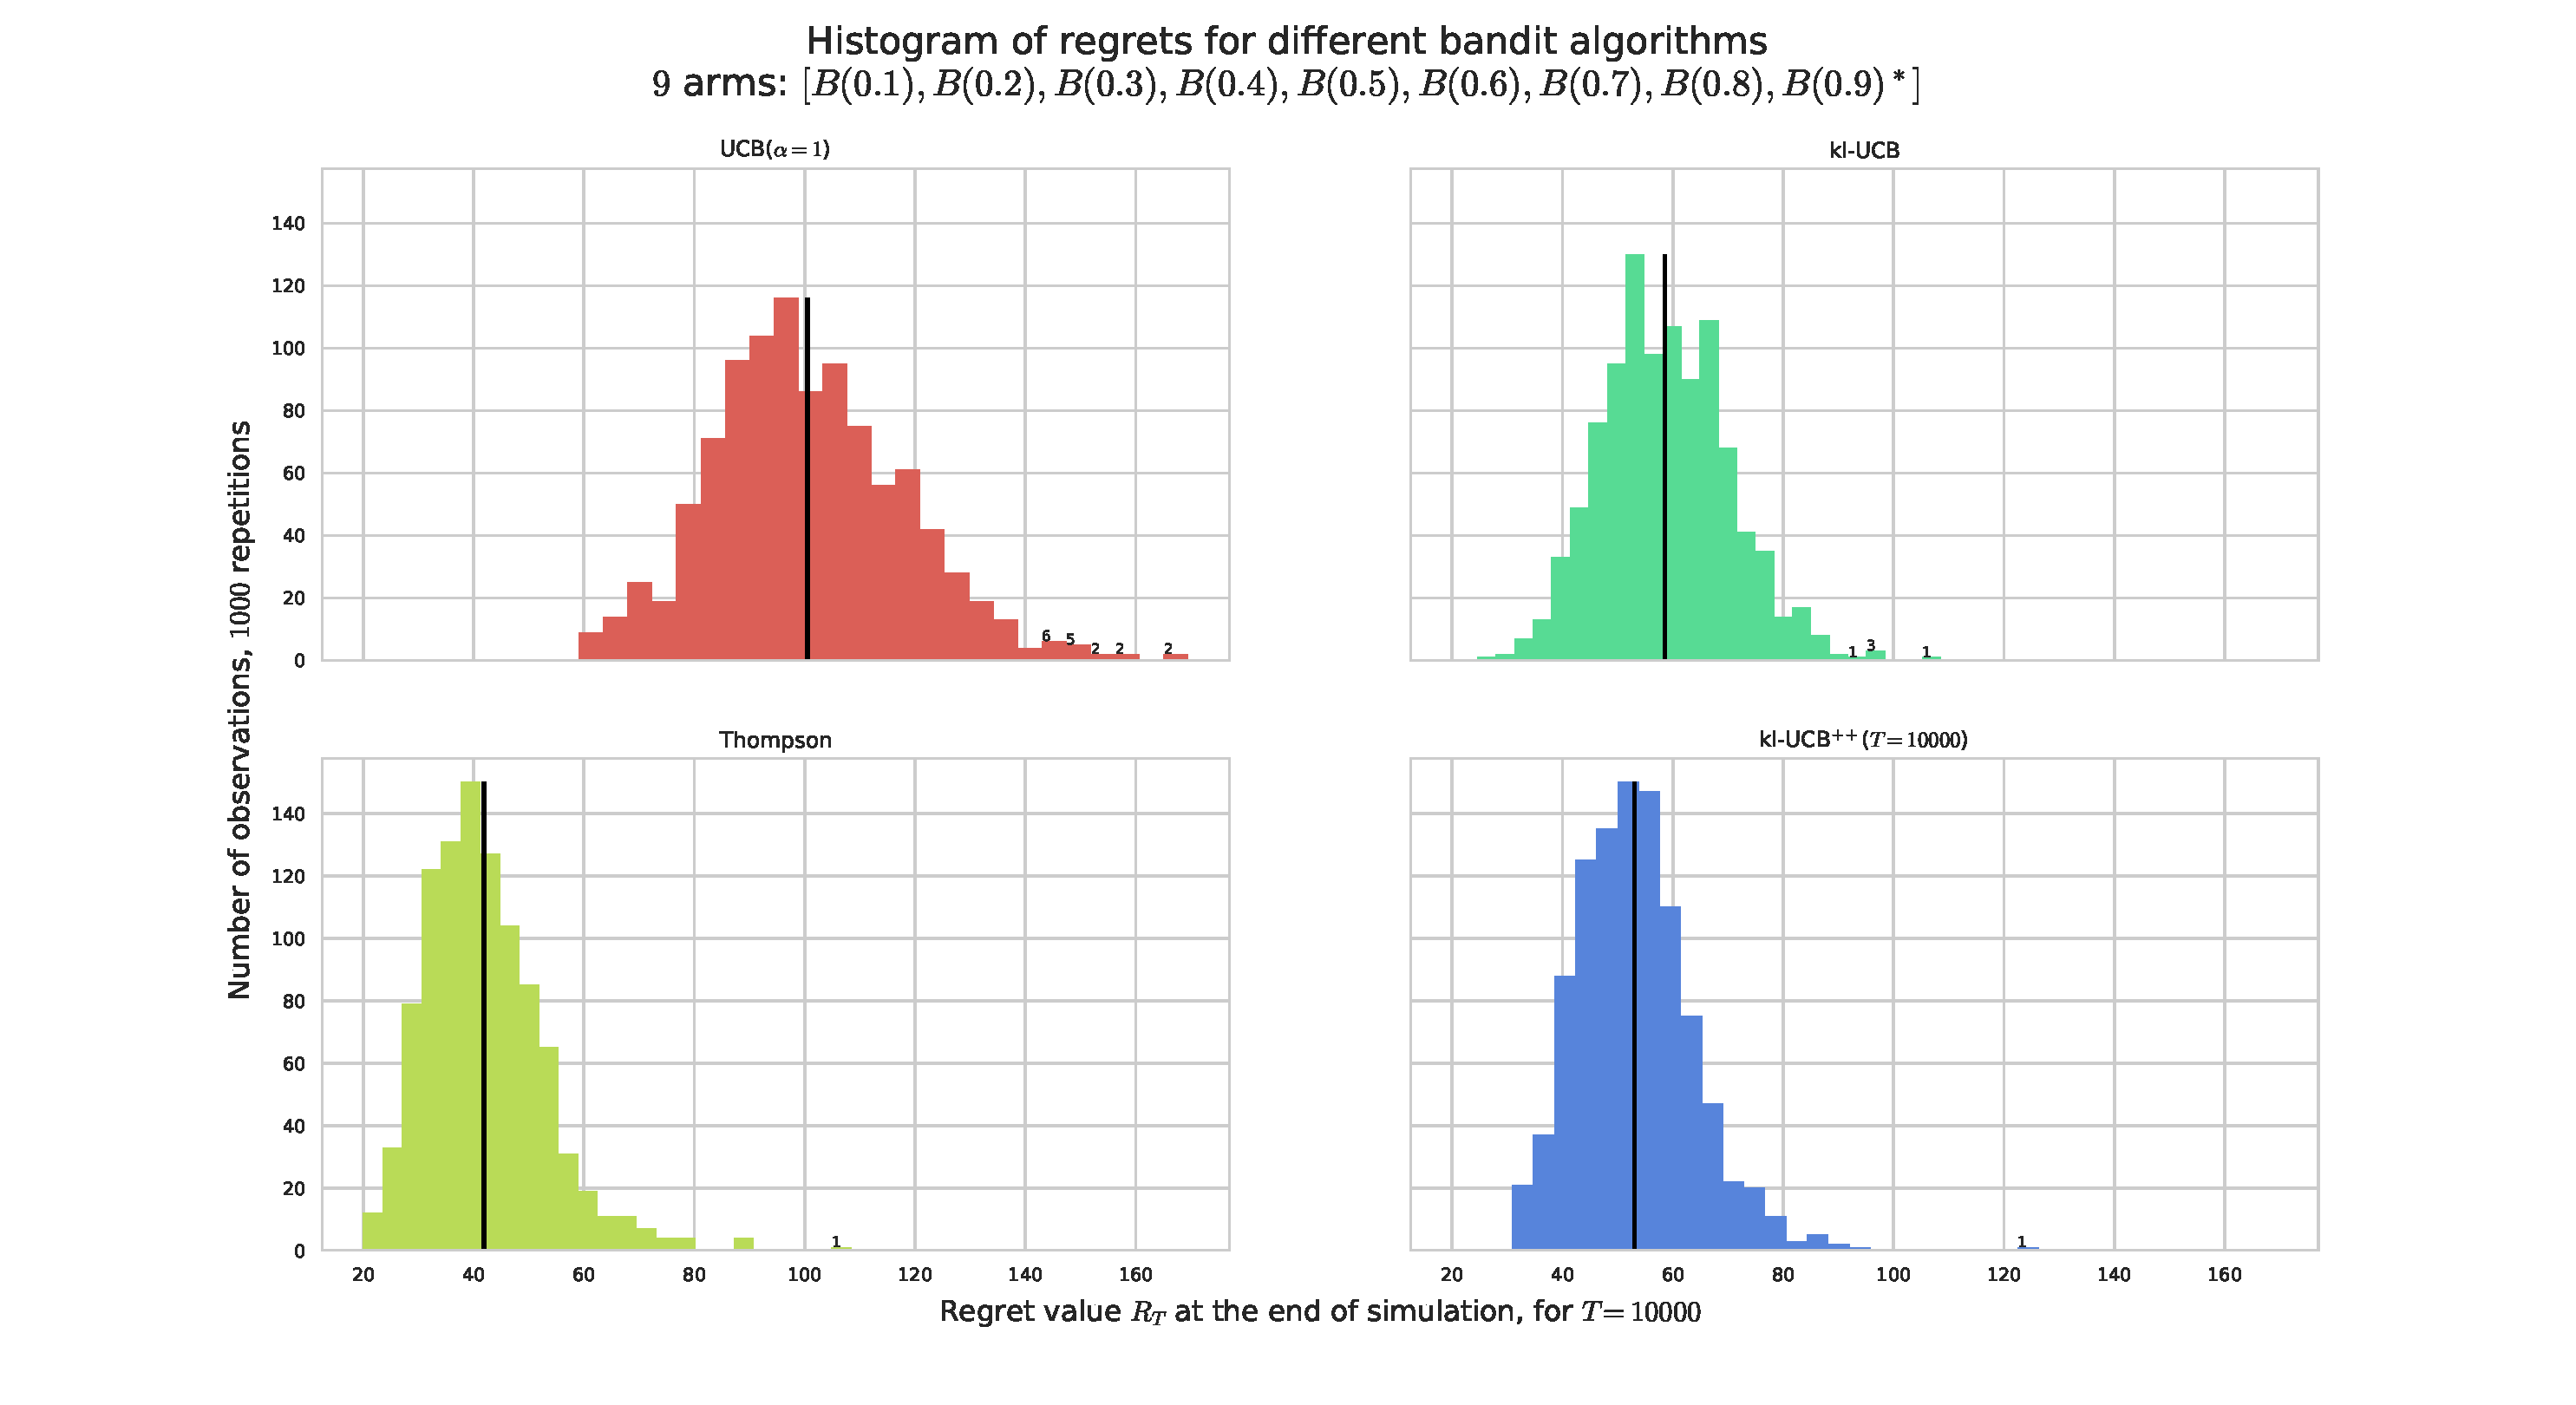
\includegraphics[width=1.05\linewidth]{3_hist.pdf}
	\caption{Histogram of regret for the same experiment.}
	\label{fig:3:firstPlot_hist}
\end{figure}


\subsection{Dependencies}

This library is written in Python \cite{python}, for versions 2.7+ or 3.4+, using \texttt{matplotlib} \cite{matplotlib} for 2D plotting, \texttt{numpy} \cite{numpy} for data storing, random number generations and operations on arrays, \texttt{scipy} \cite{scipy} for statistical and special functions, and \texttt{seaborn} \cite{seaborn} for pretty plotting and colorblind-aware colormaps.

Optional dependencies include \texttt{joblib} \cite{joblib} for parallel simulations, \texttt{numba} \cite{numba} for automatic speed-up on small functions, \texttt{sphinx} \cite{sphinx} for generating the documentation, \texttt{virtualenv} \cite{virtualenv} for launching simulations in isolated environments, and \texttt{jupyter} \cite{jupyter} used with \texttt{ipython} \cite{ipython} to experiment with the code.

All the quoted libraries are free and open-source and can be installed in one command using the \texttt{pip} (\texttt{\href{https://pip.pypa.io/}{pip.PyPa.io}}) or \texttt{conda} (\texttt{\href{http://conda.anaconda.org/}{conda.anaconda.org}}) package manager.


\subsection{Research works using SMPyBandits}

SMPyBandits was used for the following research articles since $2017$, and it is used for the next chapters of this thesis (except in Chapter~\ref{chapter:4}).

In \cite{Besson2018WCNC} and in Chapter~\ref{chapter:2} above, we used SMPyBandits to illustrate and compare different aggregation algorithms\footnote{~See the page \texttt{\href{https://SMPyBandits.GitHub.io/Aggregation.html}{SMPyBandits.GitHub.io/Aggregation.html}} on the documentation, which gives detailed instructions to reproduce the results presented in this research paper, details about the models and the notations, and bibliographic references.}. We designed a variant of the Exp4 algorithm for online aggregation of experts \cite{Bubeck12}, called \texttt{\href{https://SMPyBandits.GitHub.io/docs/Policies.Aggregator.html}{Aggregator}}.
% Aggregating experts is a well-studied idea in sequential learning and in machine learning in general. We showed that it can be used in practice to select on the run the best bandit algorithm for a certain problem from a fixed pool of experts. This idea and algorithm can have interesting impact for Opportunistic Spectrum Access applications \cite{Jouini09} that use multi-armed bandits algorithms for sequential learning and network efficiency optimization.

In \cite{Besson2018ALT} and in Chapter~\ref{chapter:5} below, we used SMPyBandits for all the simulations for multi-player bandit algorithms\footnote{~See the page \texttt{\href{https://SMPyBandits.GitHub.io/MultiPlayers.html}{SMPyBandits.GitHub.io/MultiPlayers.html}} on the documentation.}. We designed the two \texttt{\href{https://SMPyBandits.GitHub.io/docs/PoliciesMultiPlayers.RandTopM.html}{RandTopM}} and \texttt{\href{https://SMPyBandits.GitHub.io/docs/PoliciesMultiPlayers.MCTopM.html}{MCTopM}} algorithms and proved than they enjoy logarithmic regret in the usual setting, and outperform significantly the previous state-of-the-art solutions (\ie, \texttt{\href{https://SMPyBandits.GitHub.io/docs/PoliciesMultiPlayers.rhoRand.html}{rhoRand}}, \texttt{\href{https://SMPyBandits.GitHub.io/docs/Policies.MEGA.html}{MEGA}} and \texttt{\href{https://SMPyBandits.GitHub.io/docs/Policies.MusicalChair.html}{MusicalChair}}).

In \cite{Besson2018DoublingTricks}, we used SMPyBandits to illustrate and compare different "doubling trick" schemes\footnote{~See the page \texttt{\href{https://SMPyBandits.GitHub.io/DoublingTrick.html}{SMPyBandits.GitHub.io/DoublingTrick.html}} on the documentation.}. and lots of bibliographic referencesIn sequential learning, an algorithm is anytime if it does not need to know the horizon $T$ of the experiments. A well-known trick for transforming any non-anytime algorithm to an anytime variant is the ``Doubling Trick'': start with an horizon $T_0\in\mathbb{N}^*$, and when $t > T_i$, use $T_{i+1} = 2 T_i$. We studied two generic sequences of growing horizons (geometric and exponential), and we proved two theorems that generalized previous results. A geometric sequence suffices to conserve minimax regret bounds (in $R_T = \mathcal{O}(\sqrt{T})$), with a constant multiplicative loss $\ell \leq 4$, but cannot be used to conserve a logarithmic regret bound (in $R_T = \mathcal{O}(\log(T))$). And an exponential sequence can be used to conserve logarithmic bounds, with a constant multiplicative loss also $\ell \leq 4$ in the usual setting. It is still an open question to know if a well-tuned exponential sequence can conserve minimax bounds, or "weak" minimax bounds (in $R_T = \mathcal{O}(\sqrt{T \log(T)})$).

In \cite{Besson2019GLRT} and \cite{Besson2019Gretsi}, and in Chapter~\ref{chapter:6} below, we used SMPyBandits for piece-wise stationary MAB models (only for the single-player case). We illustrate and compare different algorithms designed for this family of non-stationary problems\footnote{~See the page \texttt{\href{https://SMPyBandits.GitHub.io/NonStationary.html}{SMPyBandits.GitHub.io/NonStationary.html}} on the documentation.}.
We designed the \texttt{\href{https://SMPyBandits.GitHub.io/docs/Policies.GLR_UCB.html}{GLRklUCB}} policy, and implemented most of the policies from state-of-the-art research on passively or active adaptive policies, both adversarial- or stochastic-based, designed to tackle the piece-wise stationary MAB problems.
We also implemented a large benchmark of problems.


% ----------------------------------------------------------------------------
\section{Experimental comparisons of state-of-the-art single-player algorithms}
\label{sec:3:reviewSPAlgorithms}

I want to show that SMPyBandits contains highly documented implementations of all the most important algorithms designed for stationary single-player multi-armed bandit.

I will include here formulas about the main algorithms (klUCB, MOSS, etc).
I will pick some problems (Bernoulli, Gaussian, others), with fixed means or ``Bayesian'' means (\ie, changing at each time) and I will run extensive numerical simulations to compare the main algorithms.

The take away message is: klUCB beats UCB, Thompson sampling is great too, all the others algorithms are less efficient or comparable, so we only use klUCB for all the rest of this thesis.

I will include graphs showing the mean regret $R_t$ as a function of time $t$, as well as histograms or boxplots showing the distribution of $R_T$.


% ----------------------------------------------------------------------------
\section{Some numerical experiments to compare time and memory costs of various algorithms}
\label{sec:3:timeAndMemoryCosts}

I want to show the real numerical costs in terms of computation time and storage requirement of the various algorithms for single-player bandits.

Maybe I can pick one simple problem family (\eg, evenly spaced in $[\varepsilon,1-\varepsilon]$), and run experiments for $T=1000,5000,10000$ etc, and $K=2,3,5,9,20,30,50,100,1000$ and show the evolution of time/memory as a function of $T$ and $K$.

The goal is to highlight that the simplest (but most efficient) algorithms have a memory cost bounded by $\bigO{K}$ and a time complexity at each time step $t\in[T]$ bounded by $\bigO{K}$, independent of $t$.


% % ----------------------------------------------------------------------------
% \section{An example of another model: rested or restless Markov models}
% \label{sec:3:markovModels}

% %  - FIXME maybe not included?

% Maybe if I have space at the end of this chapter, I can show another part of the library, maybe introduce the rested/restless Markov models (with maybe just one example) and show simulations in this model?

% SMPyBandits also implemented sparse MAB models (with $s<K$ arms with a mean $\mu_i>0$ and $K-s$ arms with a mean $\mu_i \leq 0$), I could also present this model, the various algorithms designed to tackle it, and some numerical experiments.


% ----------------------------------------------------------------------------
\section{Conclusion of Chapter 3}
\label{sec:3:conclusion}

In this chapter, we saw...

Future works include...




% ----------------------------------------------------------------------------
\section{Appendix for Chapter 3}
\label{sec:3:appendix}


\subsection{Minimalist example of use of SMPyBandits}

Below is presented in Listing~\ref{lst:3:exampleOfUse} a minimalist example of use of the library, to define a toy bandit problem with $K=2$ Bernoulli distributed arms (of means $\mu=0.1$ and $\mu=0.9$), one \UCB{} algorithm, and play one experiment of horizon $T=1000$.
Only the mean reward is printed at the end of the simulation.
%
With Python 3.6 this example shows that the algorithm got a mean reward very close to the optimal arm, $\hat{\mu} = 0.886 \simeq 0.9 = \mu^* = \mu_2$.
\begin{verbatim}
The UCB algorithm obtains here a mean reward = 0.886
\end{verbatim}

% https://tex.stackexchange.com/a/12430/
\begin{small}
% \begin{listing}[h!]
    \inputminted[linenos=true,numbersep=5pt,frame=lines,framesep=2mm]{python3}{2-Chapters/3-Chapter/src/example_of_use_of_SMPyBandits.py}
    % \caption{Small example of \texttt{main.py} file}
    \captionof{listing}{Example of use of SMPyBandits\label{lst:3:exampleOfUse}.}
    % \label{lst:3:exampleOfUse}
% \end{listing}
\end{small}


\subsection{A minimalist \texttt{main.py} file}

We present below in Listing~\ref{lst:3:main} a full example of a minimalist \texttt{main.py} file,
which is used to load the configuration, run the experiment and then print and plot various visualizations for the simulation.

% https://tex.stackexchange.com/a/12430/
\begin{small}
% \begin{listing}[h!]
    \inputminted[linenos=true,numbersep=5pt,frame=lines,framesep=2mm]{python3}{2-Chapters/3-Chapter/src/example_of_main_singleplayer.py}
    % \caption{Small example of \texttt{main.py} file}
    \captionof{listing}{Small example of \texttt{main.py} file\label{lst:3:main}.}
    % \label{lst:3:main}
% \end{listing}
\end{small}


\subsection{A minimalist \texttt{configuration.py} file}

We present below in Listing~\ref{lst:3:configuration} a full example of a minimalist \texttt{configuration.py} file,
which is used to define the experiment.
It defines the number of arms $K$ and their distribution, the horizon $T$, the policies to test etc.
It uses environment variables, so a user can configure some parameters of the simulation when launching them:

% \begin{verbatim}
%     (bash) $ T=50000 N=100 K=10 ARM_TYPE=Gaussian python main.py
% \end{verbatim}

% https://tex.stackexchange.com/a/12430/
\begin{listing}[h!]
    \begin{minted}[linenos=true,numbersep=5pt,frame=lines,framesep=2mm]{bash}
$ T=50000 N=100 K=10 ARM_TYPE=Gaussian python main.py
    \end{minted}
    \caption{Small snippet of Bash to run an experiment}
    % \captionof{listing}{Small snippet of Bash to run an experiment \label{lst:3:howToRunExperiment2}.}
    \label{lst:3:howToRunExperiment2}
\end{listing}

% https://tex.stackexchange.com/a/12430/
\begin{small}
% \begin{listing}[h!]
    \inputminted[linenos=true,numbersep=5pt,frame=lines,framesep=2mm]{python3}{2-Chapters/3-Chapter/src/example_of_configuration_singleplayer.py}
    % \caption{Small example of \texttt{configuration.py} file}
    \captionof{listing}{Small example of \texttt{configuration.py} file\label{lst:3:configuration}.}
    % \label{lst:3:configuration}
% \end{listing}
\end{small}


\subsection{A final note about parallelism in SMPyBandits}
\label{sub:3:parallelSimulations}
% Using multi-core to speed-up simulations

Nowadays, parallelism is everywhere in the computational world, and any serious framework for numerical simulations must explore at least one of the three main approaches to (try to) gain performance from parallelism.
%
For all the different numerical simulations presented in this thesis, except the ones based on MATLAB or GNU Radio in Chapter~\ref{chapter:4}, the setting is the same: we consider a small set of $p$ different problems, of time horizon $T$ that we want to simulate for $N$ independent runs (\eg, $p=6$, $T=10000$ and $N=100$ like in Chapter~\ref{chapter:6}).
On the first hand, because of the fundamentally sequential nature of bandit games, each repetition of the simulation must be sequential regarding the time steps $t=1,\dots,T$, and so no parallelism can be done to speed up this axis.
On the other hand, parallelism can help greatly for the two other axes: if we have a way to run in parallel $4$ processes, and we have $p=4$ problems to simulate, then running a process for each problem directly brings a speed-up factor of $4$.
Similarly, if we want to run $100$ repetitions of the same (random) problem, and we can run $4$ processes in parallel, then running $100/4=25$ repetitions on each process also bring a speed-up factor of $4$.
%
In this last section, we quickly review the chosen approach for SMPyBandits (multi-core on one machine), and we explain why the two other approaches were less appropriate for our study of multi-armed bandit problems.

\paragraph{What we did implement: \tettt{Joblib} for multi-core simulations.}
%
The first approach is to use multiple cores of the same machines, and because it is both the simplest and the less financially as well as ecologically costly, this is the approach implemented in SMPyBandits.
The machines I had access to during my thesis, either my own laptop or a workstation hosted the SCEE team in CentraleSupélec campus, were equipped with $i5$ or $i7$ Intel CPU with $4$ or $12$ cores.
%
As explained in the page \href{https://smpybandits.github.io/How_to_run_the_code.html}{\texttt{SMPyBandits.GitHub.io/How\_to\_run\_the\_code.html}}, we implemented in SMPyBandits an easy way to run any simulations on $n$ cores of a machine, using the \texttt{Joblib} \cite{joblib} library.
It is implemented in a completely transparent way, and if someone uses the command-line variable to configure experiments, using one core or all the cores of the machine one changes \texttt{N\_JOBS=1} to \texttt{N\_JOBS=-1}, like in this example.

% https://tex.stackexchange.com/a/12430/
\begin{small}
    \begin{listing}[h!]
        \begin{minted}[linenos=true,numbersep=5pt,frame=lines,framesep=2mm]{bash}
$ BAYES=False ARM_TYPE=Bernoulli N=100 T=10000 K=9 N_JOBS=1 \
  python3 main.py configuration.py
        \end{minted}
        \caption{To run such simulation using the maximum number of cores, use \texttt{N\_JOBS=-1} instead.}
        % \captionof{listing}{Run a simulation using 1 or \texttt{N} cores \label{lst:3:runOneCoreOrMore}.}
        \label{lst:3:runOneCoreOrMore}
    \end{listing}
\end{small}

As long as the number of jobs (\texttt{N\_JOBS} here) is less then or equal to the number of physical cores in the CPU of the computer, the final speed-up in terms of total computation runtime is almost optimal, dividing the running time by \texttt{N\_JOBS}.
But jobs are implemented as threads, so the speed-up cannot be more than the number of cores, and using for instance $20$ jobs on $4$-cores for the $20$ repetitions is highly sub-optimal, as the CPU will essentially spend all his time (and memory) managing the different jobs, and not actually doing the simulations.
Using the above example, we illustrate the effect of using multi-jobs and multi-cores on the time efficiency of simulations using SMPyBandits. We consider three values of \texttt{N\_JOBS}, $1$ to use only one core and one job, $4$ to use all the $4$ cores of my $i5$ Intel CPU, and $20$ jobs.
We give in Table~\ref{table:3:speedUpTimeParallelComputations}

\TODOL{Je veux terminer cet exemple!}

% FIXME run
% for N in 1 10 100; do for NJOBS in 1 4 100; do DEBUG=True SAVEALL=False NOPLOTS=True N=$N T=10000 N_JOBS=$NJOBS make single; read; done

\begin{table}[ht]
% \begin{footnotesize}
    \centering
    \begin{tabular}{c|ccc}
    \textbf{Repetitions} $\;$ \textbackslash $\;$ \texttt{N\_JOBS} & $1$ & $4$ & $20$ \\
        \hline
        $1$ repetition    & $15 \;\text{s}$ & $XXX \;\text{s}$ & $XXX \;\text{s}$ \\
        $10$ repetitions  & $87 \;\text{s}$ & $XXX \;\text{s}$ & $XXX \;\text{s}$ \\
        $100$ repetitions & $749 \;\text{s}$ & $XXX \;\text{s}$ & $XXX \;\text{s}$ \\
        $500$ repetitions & $XXX \;\text{s}$ & $XXX \;\text{s}$ & $XXX \;\text{s}$ \\
        \hline
    \end{tabular}
    \caption{Effect on the running time of using \texttt{N\_JOBS} jobs in parallel, for a simulation with $9$ different algorithms, for $K=9$ arms, a time horizon of $T=10000$.}
    \label{table:3:speedUpTimeParallelComputations}
% \end{footnotesize}
\end{table}

% Explain why I didn't try more on parallelisation (eg on Grid5000 or other large scale computer).
\paragraph{Approaches we did not try.}
%
The two other approaches we could have consider is parallel computations running on not multiple cores but multiple machines, in a computer cluster, or parallel computations running in a Graphical Processing Unit (GPU).

On the first hand, I did not try to add in SMPyBandits the possibility to run simulations using a GPU, or any general purpose computation libraries offering a GPU-backend.
Initially designed for graphical simulations and mainly for video-games applications, the use of GPU for scientific computations have been gaining attention for numerical simulation in the research world since the last $15$ years, and NVidia CUDA for GPGPU (General Purpose GPU) started to become popular in $2011$.
Since $2016$, we saw a large press coverage as well as an extensive use in research of deep learning libraries that make general-purpose machine learning algorithms train on the GPU of a user's laptop or a cluster of GPU.
This success is mainly possible because of the heavy parallelism of such training algorithms, and the parallel nature of GPU.
To the best of the author knowledge, nobody has tried to implement high performance MAB simulations by using the ``parallelism power'' of a GPU (at least, no code for such experiments were made public in $2019$).
I worked on a GPU, implementing fluid dynamic simulations in an internship in $2012$, and I have since then kept a curiosity on how to use GPU-powered libraries and code.
I have contributed to and used famous deep-learning libraries, like Theano (\href{http://deeplearning.net/software/theano/}{\texttt{DeepLearning.net/software/theano}}) or Keras (\href{https://keras.io/}{\texttt{keras.io}}), and my limited knowledge on such libraries made me believe that it was not easy to use a GPU for bandit simulations, and most surely it would not have been worth the time.
I would be very curious to understand how a GPU could be used to implement highly efficient simulations for sequential learning problems, because it seemed hard whenever I thought about it.

On the other hand, I also did not try to use any large scale computer cluster, even if I was aware of the possibility offered by the Grid 5000 project, for instance.
It is partly due to time constraint, as I would have been curious to try, but mainly because we found that it would not have helped us much to use a large scale cluster.
The main reason is that in the multi-armed bandit and sequential learning literature, most research papers do not even include an experimental section, and for the papers who did take the time to implement and test their proposed algorithms, it is almost done on just a few problems and for short- or medium- duration experiments.
For instance, the papers we consider to be the best ones regarding their empirical sections are \cite{LiuLeeShroff17,CaoZhenKvetonXie18}, for piece-wise stationary bandits, and they mainly consider reasonable problems of horizon $T=10000$ and no more than $1000$ independent repetitions. Each paper considers one harder problem, of horizon $T=1000000$ and less repetitions.
%
In each article written during my thesis, we included extensive numerical simulations, and even the longest ones (for \cite{Besson2019GLRT}) were short enough to run in less than $12$ hours on a $12$-core workstation, so we could run a few large-scale simulations over night.
For such reasons, we prefer to not try to run simulations on a cluster.
